\documentclass[preprint,12pt,a4paper]{elsarticle}
\usepackage[margin=25mm]{geometry}
\usepackage{amsmath,amssymb,booktabs,tabularx,array,microtype,placeins}
\usepackage[T1]{fontenc}
\usepackage{tikz}
\usetikzlibrary{arrows.meta,positioning}
\usepackage[hyphens]{url}
\usepackage{xurl}
\usepackage[hidelinks]{hyperref}
\newcommand{\SourceRevision}{8533214105aad0cc015ea1e1c2aad4057515aff7}
\newcommand{\Repo}{https://github.com/guyoverclocked/orchlang-compiler-design-project}
\newcommand{\codepath}[1]{\nolinkurl{#1}}
\journal{Science of Computer Programming}
\renewcommand{\today}{14 October 2026}
\setlength{\emergencystretch}{2em}
\makeatletter
\def\ps@pprintTitle{%
  \let\@oddhead\@empty\let\@evenhead\@empty
  \def\@oddfoot{\footnotesize\itshape Draft for Science of Computer Programming\hfill 14 October 2026}%
  \let\@evenfoot\@oddfoot}
\makeatother
\begin{document}
\begin{frontmatter}
\title{OrchLang: Replayable Analysis of Request and Usage Observations in Restricted LLM Workflows}
\author{[Author names to be supplied]}
\address{[Affiliations and correspondence to be supplied]}
\begin{abstract}
OrchLang analyzes restricted workflows containing large language model calls. It distinguishes abstract request equality, ordered usage-law equality, and bounded trace distance under explicitly supplied uncertainty contracts. The software combines a C++ compiler, rational graph analyzers and certificate replay with optional LangGraph execution. A normalized-IR Coq proof covers returned-state commits and finite routed prefixes. An exact finite uncertainty prototype improves a conservative distance bound from 1 to 1/2 in a separating example. Evaluation includes 104 authored source/backend comparisons, two bounded public-source slices, and 27 structured scaling cases. A disjoint source cohort admits none of nine candidates, delimiting current applicability. Provider calibration and independent human reproduction remain pending.
\end{abstract}
\begin{keyword}
workflow analysis \sep information flow \sep resource observations \sep probabilistic traces \sep certificate replay \sep research software
\end{keyword}
\end{frontmatter}

\section{Motivation and significance}
A workflow can hide a secret in its returned text while revealing it through which model is called, the order of calls, or their resource usage. Equal aggregate totals also need not imply equal ordered observations. OrchLang makes these distinctions executable: a user supplies a restricted workflow or request graph, fixes public inputs, enumerates secret scenarios, and selects an observation and model contract. The result is an analysis of that declared model.

The contribution is software that connects request-sensitive relational checks, exact finite-state usage-law comparison and replayable finite uncertainty contracts. It specializes established methods rather than claiming a new general verification algorithm. Relational cost analysis already compares program costs~\cite{relcost}; weighted-automaton methods decide rational language equivalence~\cite{kiefer}; imprecise probability and total-variation ambiguity provide the uncertainty setting~\cite{cooman,tzortzis}. Recent PPDL work models uncertain LLM flows~\cite{ppdl}, while typed-resources checks sequential workflow ceilings~\cite{typed}. OrchLang instead exposes a selected relational usage observer and keeps its source, probability and execution premises separate. The technical supplement gives the semantic argument and a focused comparison with adjacent workflow-assurance systems.

\section*{Metadata}
\begingroup\small
\renewcommand{\arraystretch}{1.13}
\noindent\begin{tabularx}{\textwidth}{@{}l >{\raggedright\arraybackslash}p{4.3cm} >{\raggedright\arraybackslash}X@{}}
\toprule
Nr. & Code metadata description & Information for this candidate \\
\midrule
C1 & Current code version & 0.5.0rc3 \\
C2 & Permanent link to code/repository used for this code version & \href{\Repo/tree/\SourceRevision}{Immutable Git revision 8533214}; full SHA in supplement. \\
C3 & Permanent link to Reproducible Capsule & Persistent archive/capsule identifier pending; local source and evidence ZIPs prepared. \\
C4 & Legal Code License & MIT; retained third-party source notices/licenses. \\
C5 & Code versioning system used & Git \\
C6 & Software code languages, tools, and services used & C++17, Python, Coq/Rocq; optional LangGraph. Offline analysis needs no provider service. \\
C7 & Compilation requirements, operating environments and dependencies & C++17 compiler and make; Python 3.11/3.14 tested. Optional runtime: LangGraph 1.2.14, LangChain Core 1.6.9; proof build: \texttt{coqc}. \\
C8 & If available, link to developer documentation/manual & \href{\Repo/blob/\SourceRevision/docs/SCP_STRENGTHENING.md}{Candidate documentation and reproduction commands}. \\
C9 & Support email for questions & [Author confirmation required] \\
\bottomrule
\end{tabularx}
\endgroup

\section{Software description}
\subsection{Architecture}
The compiler checks types, labels, bounded costs and paired abstract call descriptors. Python tools analyze normalized request graphs and supplied rational outcome kernels; separate replay tools check closures, equality certificates or finite witnesses. A bounded Python AST frontend admits a small StateGraph fragment. Optional execution uses actual LangGraph with an offline oracle. Two additional research prototypes consume uncertainty contracts directly; they are separate from the eight installed graph commands.

\begin{figure}[h]
\centering
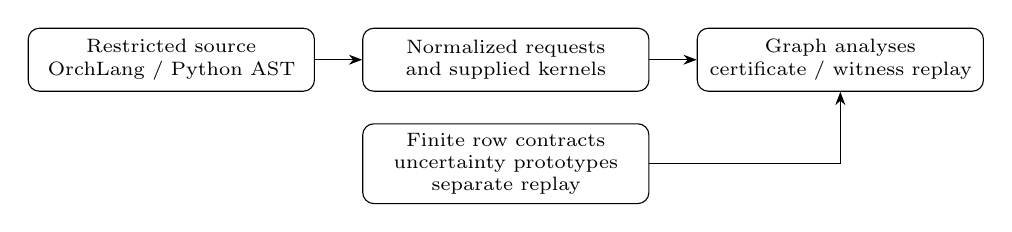
\begin{tikzpicture}[font=\scriptsize,box/.style={draw,rounded corners,align=center,text width=3.4cm,minimum height=0.8cm},>=Stealth]
\node[box] (src) {Restricted source\\OrchLang / Python AST};
\node[box,right=0.6cm of src] (ir) {Normalized requests\\and supplied kernels};
\node[box,right=0.6cm of ir] (cert) {Graph analyses\\certificate / witness replay};
\draw[->] (src)--(ir); \draw[->] (ir)--(cert);
\node[box,below=0.4cm of ir] (row) {Finite row contracts\\uncertainty prototypes\\separate replay};
\draw[->] (row.east)-|(cert.south);
\end{tikzpicture}
\caption{Inputs and checking boundaries. Extraction and provider-model validity are premises outside the normalized-IR proof.}
\end{figure}

\subsection{Functionality and guarantees}
An abstract call key contains a resolved model contract, decoded template bytes, ordered argument values and the contract's invocation ordinal. Matching keys under a shared deterministic oracle supports paired request/response behavior. This descriptor omits provider-added framing and SDK serialization. Input usage follows the declared additive UTF-8 byte-divisor estimator; its units are modeled usage, not measured provider tokens or invoices.

For a closed finite rational kernel, exact row-span analysis decides success-only ordered usage-law equality for every finite horizon, at the supplied public store and secret scenarios. Stop and live prefix masses are separate outputs. A distinguishing word witnesses inequality; resource exhaustion yields \texttt{UNKNOWN}. Kernel history retention and ordinal saturation at 33 are explicit parts of this abstraction.

The new finite uncertainty prototype instead accepts, at every scenario and full visible prefix, a convex hull of rational conditional rows. Independent choices across rows and scenarios are required. For prefix masses $a,b$, its minimum suffix overlap is
\[
C_h(a,b)=\min_{p_0,p_1}\sum_y C_{hy}(a p_0(y),b p_1(y)),
\qquad C_H(a,b)=\min(a,b).
\]
Trace TV is an established comparison~\cite{chen}. Here its maximum over the declared rectangular contract is $1-C_{\epsilon}(1,1)$. Concavity permits enumeration of supplied generator pairs; the replay derives all subproblems and recomputes their minima. STOP is visible and padded. Unless universal stopping is checked, the result covers only the bounded prefix. This exact finite contract is different from an inferred provider distribution.

\section{Illustrative examples}
In the two-slot singleton-row (fixed-kernel) fixture, both scenarios emit $A$ or $B$ with probability $1/2$. After $A$, their second symbols are respectively $C$ and $D$; after $B$, both emit $C$. Their trace laws are $\{AC:1/2,BC:1/2\}$ and $\{AD:1/2,BC:1/2\}$. Exact TV is $1/2$. A conservative pathwise coupling bound takes the worst continuation and returns 1. Preserving probability masses therefore matters even in this small example; the artifact contains the contract, certificate and exhaustive reference checks.

A three-call authored node produces a returned draft, an internal critique and a returned answer. In the recorded UTF-8 example, modeled input/output units are $(8,5)$, $(9,8)$ and $(15,6)$. Source state commits only the draft and answer. Backend format 2 exposes completed registers for projection to those fields; on a cutoff or failure it returns \codepath{final_values=null}, preventing partial eager writes from masquerading as a completed source state.

\section{Evaluation}
The source revision was frozen before a 19-stage offline reproduction, which passed with source fingerprints checked before and after execution. Six CI jobs passed, including Linux/macOS core checks with Python 3.11/3.14, an Ubuntu proof build, and the pinned LangGraph study. The local run passed 112 native regressions, 230 audit tests, 22 frontend tests, 23 conservative-contract tests, 21 exact-contract tests, 19 fake-transport tests, 14 capsule-verifier tests, 11 backend tests and eight state-review tests; the wheel passed 23 isolated validation stages. These are implementation checks, not a proof of the full software stack.

\begin{table}[h]
\small\centering
\begin{tabularx}{\textwidth}{@{}>{\raggedright\arraybackslash}p{3.4cm} >{\raggedright\arraybackslash}X@{}}
\toprule
Evidence object & Observed result and scope \\
\midrule
Normalized IR & Returned-state and finite routed-prefix refinement; seven closed-context reports. AST extraction and initialization remain bridge obligations. \\
Authored workflows & 96 completed and eight cutoff pairs; 224 events; trace/status/completed-state comparisons pass. A separate 18-case truth table exercises both outcomes of six token comparisons. \\
Finite contracts & 26 development contracts, 20,739 complete-law pairs, no mismatch; fresh separate oracle: 120 contracts, 1,888 pairs and 120 attaining witnesses. \\
Public source slices & Two recorded bounded slices, six and 12 schedules. Fresh reproduction replays their recorded finite models, without executing original source again. \\
Source admission & Development: 0/59 candidates. Disjoint holdout: 0/9; 11/12 repositories retrieved, 1,580 Python paths. One retrieval-cap failure is retained. \\
\bottomrule
\end{tabularx}
\caption{Different evidence classes have different subjects and premises.}
\end{table}
\FloatBarrier

Selected hash-pinned original statements and callables were previously executed with actual pinned LangGraph and explicit offline boundary doubles. Their complete recorded finite laws have six and 12 trace classes, versus four content-only and two final-answer classes in each capsule. Separate replay checks the declared schedules and projections exactly; it does not independently witness the source execution.

The structured synthetic matrix covers 27 cases over branches, public context, mutable registers, cycles, response support, observation alphabet and retained history: 122 operation/version groups, 732 raw rows and 610 measured rows. Current exact analysis gives 25 equal cases, one unequal case and one resource-limited case, each repeated five times. Completed closure sizes range from 4 to 190; the largest completed exact producer/replay medians are 77.53/164.82 ms. UNKNOWN stop times remain raw diagnostics and are excluded from completed-result latency. The final reproduction validates these recorded timings; it does not rerun the timing study.

\section{Impact and limitations}
OrchLang provides inspectable experiments for questions that aggregate accounting can obscure: whether ordered resource observations distinguish secret alternatives, whether trace equality holds despite a failed bisimulation proof, and how conditional row uncertainty changes bounded distinguishability. Its demonstrated use is the research suite reported here. No independent adoption, production deployment or downstream scientific impact is claimed.

The holdout's zero admission is a substantive limitation, not an extraction success. All nine candidates first reject at import handling. The two public-source capsules demonstrate bounded execution of selected immutable slices with mocks; they do not increase whole-file admission coverage. Their six and 12 equally weighted schedules are authored experimental distributions. Full trace observations retain status, messages and declared metadata, while content-only projections intentionally collapse distinctions.

Following standard compiler simulation methods~\cite{leroy}, the Coq theorem relates paired normalized nodes under read-safety, unique, completely produced returns and route correspondence. It covers finite node prefixes including cycles, not termination, arbitrary Python, the actual extractor or provider behavior. Certificate replay also retains trusted code: the exact prototype shares parsing and arithmetic; the conservative prototype shares local semantic helpers. The latter's fault-injection study shows how a shared helper defect can defeat both traversals. These boundaries remain adjacent to the claims they qualify.

Provider request serialization, empirical probability rows, retries, billing and external tokenizer bounds are unvalidated. The offline API harness is prepared for a small descriptive calibration, with no paid calls performed. Even authorized samples would not establish future row-set coverage. Usage equality also leaves cache timing outside the protected observer~\cite{cache}. Independent human reproduction and a persistent archive identifier are pending.

\section{Conclusions}
The current software makes several conditional analyses usable and replayable, with a concrete improvement in finite uncertain trace distance and stronger returned-state evidence. Its value is the explicit observation model and evidence chain. Broader extraction coverage and validated external request boundaries are necessary before applying its results to unrestricted deployed workflows.

\section*{Declarations and availability}
Code and recorded data: immutable revision linked in metadata; new paper/PDF and final-run archives are companion evidence. Author identities, CRediT roles, correspondence, funding and competing-interest declarations are placeholders requiring author completion. Codex and GPT-6 Luna agents at maximum reasoning assisted implementation, investigation and drafting. Final human review, responsibility and approval have not yet been recorded. No journal submission or acceptance is asserted. The standalone technical supplement contains proofs, assumptions, case protocols, resource limits, provenance and reproduction instructions.

\newpage
\begin{thebibliography}{9}
\bibitem{relcost} E. \c{C}i\c{c}ek, G. Barthe, M. Gaboardi, D. Garg, J. Hoffmann, Relational cost analysis, POPL (2017). \href{https://doi.org/10.1145/3009837.3009858}{doi:10.1145/3009837.3009858}.
\bibitem{kiefer} S. Kiefer, A. S. Murawski, J. Ouaknine, B. Wachter, J. Worrell, Language equivalence for probabilistic automata, CAV (2011), 526--540. \href{https://doi.org/10.1007/978-3-642-22110-1_42}{doi:10.1007/978-3-642-22110-1\_42}.
\bibitem{cooman} G. de Cooman, F. Hermans, E. Quaeghebeur, Imprecise Markov chains and their limit behaviour, Probability in the Engineering and Informational Sciences (2009). \href{https://doi.org/10.1017/S0269964809990039}{doi:10.1017/S0269964809990039}.
\bibitem{tzortzis} I. Tzortzis, C. D. Charalambous, T. Charalambous, Dynamic programming subject to total variation distance ambiguity, SIAM Journal on Control and Optimization (2015). \href{https://doi.org/10.1137/140955707}{doi:10.1137/140955707}.
\bibitem{ppdl} L. Mandel, G. Baudart, M. Vaziri, M. Hirzel, PPDL: LLM-Based Flows as Probabilistic Programs, ICML, PMLR 306 (2026), 86172--86197. \href{https://proceedings.mlr.press/v306/mandel26a.html}{Publisher record}.
\bibitem{typed} H. Inverso, A Lean-Checked Potential Calculus for Bounded-Cost LLM-Agent Workflows: A Sequential Core, preprint v4 (12 June 2026); software revision 9ef2ee9. \href{https://doi.org/10.5281/zenodo.20663552}{Version record}.
\bibitem{chen} T. Chen, S. Kiefer, On the total variation distance of labelled Markov chains, LICS (2014). \href{https://doi.org/10.1145/2603088.2603099}{doi:10.1145/2603088.2603099}.
\bibitem{leroy} X. Leroy, Formal verification of a realistic compiler, Communications of the ACM 52(7) (2009), 107--115. \href{https://xavierleroy.org/publi/compcert-CACM.pdf}{Author manuscript}.
\bibitem{cache} C. Gu, X. L. Li, R. Kuditipudi, P. Liang, T. Hashimoto, Auditing Prompt Caching in Language Model APIs, ICML, PMLR 267 (2025), 20477--20496. \href{https://proceedings.mlr.press/v267/gu25b.html}{Publisher record}.
\end{thebibliography}
\end{document}
